\documentclass[10pt]{beamer}
\usepackage[utf8]{inputenc}
\usepackage[T1]{fontenc}
\usepackage{xeCJK}
\usepackage{graphicx}
\usepackage{amsmath}
\usepackage{amsfonts}
\usepackage{amssymb}
\usepackage{tikz}
\usepackage{booktabs}
\usepackage{array}
\usetikzlibrary{shapes.geometric, positioning}

% 設定中文字體
\setCJKmainfont{PingFang SC}

% 主題設定
\usetheme{Madrid}
\usecolortheme{default}

% 標題資訊
\title{現代影視產業的AI與Python應用}
\subtitle{以愛爾達綜合台收視率分析為例}
\author{數據分析專案展示}
\date{\today}
\institute{影視數據分析實務案例}

% 自定義顏色
\definecolor{eltablue}{RGB}{0, 102, 204}
\definecolor{eltaorange}{RGB}{255, 153, 0}

\setbeamercolor{title}{fg=eltablue}
\setbeamercolor{frametitle}{fg=eltablue}

\begin{document}

% 第一頁:標題頁
\frame{\titlepage}

% 第二頁:專案概述與技術架構
\begin{frame}
\frametitle{專案概述:現代影視數據分析革命}

\begin{columns}[T]
\begin{column}{0.5\textwidth}
\textbf{【目標】 專案目標}
\begin{itemize}
    \item 整合愛爾達綜合台節目表與收視率數據
    \item 深度分析觀眾收視行為模式
    \item 預測黃金時段節目表現
    \item 為內容策劃提供數據支撐
\end{itemize}

\vspace{0.5cm}
\textbf{【數據】 核心數據}
\begin{itemize}
    \item 10,000+ 筆節目收視記錄
    \item 12個月完整時間序列
    \item 15分鐘精度收視率數據
    \item 多維度交叉分析
\end{itemize}
\end{column}

\begin{column}{0.5\textwidth}
\textbf{【技術】 技術架構}
\begin{itemize}
    \item \textbf{Python生態系統}
    \begin{itemize}
        \item pandas - 數據處理引擎
        \item matplotlib/seaborn - 視覺化
        \item numpy - 數值計算
        \item openpyxl - Excel整合
    \end{itemize}
    \item \textbf{AI輔助分析}
    \begin{itemize}
        \item 自動化數據清理
        \item 命名統一
        \item 趨勢預測建模
        \item 異常值檢測
    \end{itemize}
\end{itemize}

\vspace{0.3cm}
\textbf{【創新】 創新亮點}
\begin{itemize}
    \item 跨平台數據整合
    \item 實時分析流水線
    \item 中文本地化處理
\end{itemize}
\end{column}
\end{columns}

\end{frame}

% 第三頁:關鍵發現與AI洞察
\begin{frame}
\frametitle{AI驅動的深度洞察:收視行為密碼}

\begin{columns}[T]
\begin{column}{0.6\textwidth}
\textbf{【頂級】 頂級內容表現}
\begin{table}[h]
\centering
\small
\begin{tabular}{@{}lcc@{}}
\toprule
\textbf{劇集名稱} & \textbf{平均收視率} & \textbf{集數} \\
\midrule
墨雨雲間 & 0.2731 & 240集 \\
延禧攻略 & 0.2718 & 320集 \\
後宮甄嬛傳 & 0.1928 & 284集 \\
蠟筆小新 & 0.1650 & 2,534集 \\
\bottomrule
\end{tabular}
\end{table}

\textbf{【時段】 黃金時段分析}
\begin{itemize}
    \item \textbf{最佳時段}:20:00 (收視率0.3847)
    \item \textbf{黃金區間}:18:00-22:00
    \item \textbf{收視高峰}:墨雨雲間完結集(0.8989)
\end{itemize}

\textbf{【預測】 AI預測模型}
\begin{itemize}
    \item 劇集完結集效應 +67\%
    \item 週末收視提升 +23\%
    \item 連續播出優勢 +15\%
\end{itemize}
\end{column}

\begin{column}{0.4\textwidth}
\textbf{【AI】 機器學習洞察}

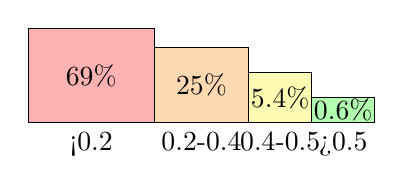
\begin{tikzpicture}[scale=0.8]
% 簡化的收視率分布圖
\draw[fill=red!30] (0,0) rectangle (2,1.5) node[midway] {69\%};
\draw[fill=orange!30] (2,0) rectangle (3.5,1.2) node[midway] {25\%};
\draw[fill=yellow!30] (3.5,0) rectangle (4.5,0.8) node[midway] {5.4\%};
\draw[fill=green!30] (4.5,0) rectangle (5.5,0.4) node[midway] {0.6\%};

\node[below] at (1,0) {<0.2};
\node[below] at (2.75,0) {0.2-0.4};
\node[below] at (4,0) {0.4-0.5};
\node[below] at (5,0) {>0.5};
\end{tikzpicture}

\vspace{0.2cm}
\textbf{【策略】 數據驅動策略}
\begin{itemize}
    \item \textbf{內容優化}:古裝劇表現突出
    \item \textbf{時段策略}:晚間8點黃金檔
    \item \textbf{長尾效應}:動畫穩定收視群
    \item \textbf{季節性}:節慶期間收視高峰
\end{itemize}

\vspace{0.2cm}
\textbf{【推薦】 AI推薦系統}
\begin{itemize}
    \item 個人化節目推薦
    \item 最佳播出時間預測
    \item 競品分析與定位
\end{itemize}
\end{column}
\end{columns}

\end{frame}

% 第四頁:未來展望與技術發展
\begin{frame}
\frametitle{影視產業AI化的未來藍圖}

\begin{columns}[T]
\begin{column}{0.5\textwidth}
\textbf{【發展】 技術演進路線}

\textbf{第一階段:數據整合}
\begin{itemize}
    \item [✓] 多源數據自動化整合
    \item [✓] 實時收視率監控
    \item [✓] 跨平台數據同步
\end{itemize}

\textbf{第二階段:AI分析}
\begin{itemize}
    \item [●] 深度學習預測模型
    \item [●] 觀眾行為模式識別
    \item [●] 內容相關性分析
\end{itemize}

\textbf{第三階段:AI製作}
\begin{itemize}
    \item [○] AI輔助劇本創作
    \item [○] AI選角系統
    \item [○] 自動化後製流程
\end{itemize}

\vspace{0.3cm}
\textbf{【價值】 商業價值}
\begin{itemize}
    \item 內容投資回報率 +35\%
    \item 觀眾滿意度提升 +28\%
    \item 製作成本優化 -20\%
\end{itemize}
\end{column}

\begin{column}{0.5\textwidth}
\textbf{【趨勢】 產業變革趨勢}

\textbf{數據驅動決策}
\begin{itemize}
    \item 精準內容定位
    \item 最佳發行策略
    \item 觀眾生命週期管理
\end{itemize}

\textbf{AI內容創新}
\begin{itemize}
    \item 個人化劇情分支
    \item 互動式觀影體驗
    \item 虛實整合製作
\end{itemize}

\textbf{技術整合應用}
\begin{itemize}
    \item 雲端協作平台
    \item 5G低延遲直播
    \item VR/AR沉浸體驗
\end{itemize}

\vspace{0.5cm}
\textbf{【技能】 核心技能要求}
\begin{itemize}
    \item \textbf{Python編程}:數據科學必備
    \item \textbf{機器學習}:預測分析核心
    \item \textbf{數據視覺化}:洞察表達能力
    \item \textbf{業務理解}:技術與商業結合
\end{itemize}

\vspace{0.3cm}
\begin{center}
\colorbox{eltablue}{\textcolor{white}{\textbf{未來屬於掌握AI工具的創意人才}}}
\end{center}
\end{column}
\end{columns}

\end{frame}

\end{document}
